\chapter{Проектирование дискретных стабилизирующих регуляторов.}
\label{ch:chap1}


\section{Исходные данные}
Тип объекта управления, представлен на рисунке \ref{1_schem}.
\begin{figure}[h]
\center{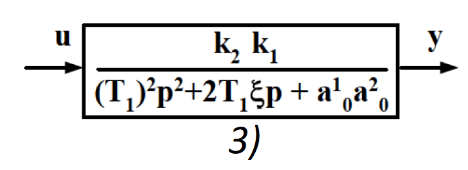
\includegraphics[width=0.75\linewidth]{pic/1_schem.png}}
\caption{Исследуемый объект управления.}
\label{1_schem}
\end{figure}

Параметры объекта управления: $k_1 =3.26$, $a_0^1 = 1$, $T_1 = 9.5$, $\xi = 0.36$, $k_2 = 1$, $a_0^2 = 1$, $T_2 = 0$, $T = 1$.

Параметры задающего воздействия: $g_0 = 2.8$, $g_1 = 0$, $A_g = 0$, $\omega_g = 0$.

\section{Ход работы}

Запишем передаточную функцию объекта управления (рисунок \ref{1_schem})
\begin{equation}
	W(p) = \frac{k_2k_1}{T_1^2p^2+2T_1\xi p + a_0^1a_0^2} = \frac{k_2k_1 /T_1^2 }{ p^2 + \frac{2\xi}{T_1}p + \frac{a_0^1a_0^2}{T_1^2}}
\end{equation}
Найдем матрицы канонической управляемой формы:
\begin{equation}
	A_c = \begin{bmatrix}
		0 & 1\\
		-a_0 & -a_1
	\end{bmatrix} = \begin{bmatrix}
	0 & 1\\
	-\frac{a_0^1a_0^2}{T_1^2} & -\frac{2\xi}{T_1}
	\end{bmatrix} =
	\begin{bmatrix}
		0 & 1\\
		-0.0111 & -0.0758
	\end{bmatrix}
\end{equation}
\begin{equation}
	B_c = \begin{bmatrix}
		0\\1
	\end{bmatrix}, \, \, 
	C = \begin{bmatrix}
		b_0 & b_1
	\end{bmatrix} = \begin{bmatrix}
	k_2k_1 /T_1^2 & 0
	\end{bmatrix} = \begin{bmatrix}
	0.0361 & 0
	\end{bmatrix}
\end{equation}

Теперь перейдем к соответствующей дискретной системе в пространстве состояний
\begin{equation}
	\begin{cases}
		x(k+1) = Ax(k) + Bu(k)\\
		y(k) = Cx(k)
	\end{cases}
\end{equation}

Найдем дискретное представление матриц $A$ и $B$ с учетом $T = 1$:
\begin{equation}
	A = \sum \limits_{i=0}^k \frac{A_c^iT^i}{i!} =
	\begin{bmatrix}
		0.9946&	0.9613\\
		-0.0107&	0.9217
	\end{bmatrix}
\end{equation}
\begin{equation}
	B = \sum \limits_{i=1}^k \frac{A_c^{i-1}T^i}{i!}B_c =
	\begin{bmatrix}
		0.4872\\
		0.9613
	\end{bmatrix}
\end{equation}

Проверим структурные свойства объекта управления.
Для проверки управляемости найдем корни характеристического полинома объекта управления и сравним модули этих чисел с единицей
\begin{equation}
	z_{1,2} = 0.9582 \pm 0.0944i \Rightarrow \|z_{1, 2} \| = 0.9628 < 1
\end{equation}
Так как собственные числа по модулю меньше единицы, то система является устойчивой, так как выполнен корневой критерий.

Для анализа управляемости системы составим матрицу управляемости и найдем её ранг
\begin{equation}
	U = \begin{bmatrix}
		B & AB
	\end{bmatrix} = \begin{bmatrix}
	0.4872 &	1.4086\\
	0.9613 &	0.8809
	\end{bmatrix} \Rightarrow rank\left(U\right) = 2,
\end{equation}
так как ранг совпал с размерностью системы, то система является полностью управляемой.

Для анализа наблюдаемости построим матрицу наблюдаемости системы и найдем ее ранг
\begin{equation}
	V = \begin{bmatrix}
		C\\
		CA
	\end{bmatrix} = \begin{bmatrix}
	0.0361 &	0\\
	0.0359 &	0.0347
	\end{bmatrix} \Rightarrow rank \left(V\right) = 2,
\end{equation}
ранг матрицы наблюдаемости равен размерности системы, следовательно, система полностью наблюдаема.

Теперь перейдем к рассчету матрицы линейных стационарных обратных связей методом модального управления. В качестве эталонной модели возьмем оптимальную по быстродействию дискретную систему, то есть примем $z_i^* = 0$, $i = \overline{1, n}$.
\begin{equation}
	\xi(k+1) = \Gamma \xi(k)\\
	y(k) = H \xi(k),
\end{equation}
где $\xi(k)$ -- вектор состояния дискретной эталонной модели.

Запишем требуемые матрицы $\Gamma$ и $H$:
\begin{equation}
	\Gamma = \begin{bmatrix}
		z_1 & 1\\
		0 & z_2
	\end{bmatrix} = \begin{bmatrix}
	0 & 1\\
	0 & 0
	\end{bmatrix}, \, \, 
	H = \begin{bmatrix}
		1 & 0
	\end{bmatrix}
\end{equation}
Проверим, что пара матриц $\left(H, \Gamma \right)$ является полностью наблюдаемой, для этого вновь составим матрицу наблюдаемости и убедимся, что её ранг равен двум
\begin{equation}
	V_{H,\Gamma} = \begin{bmatrix}
		1 & 0\\
		0 & 1
	\end{bmatrix} \Rightarrow rank \left(V_{H,\Gamma}\right) = 2
\end{equation}
Определим эталонный характеристический полином
\begin{equation}
	D^*(z) = det \{zI - \Gamma\} = z^2
\end{equation}

Теперь решим уравнение Сильвестра относительно $P$ и вычислим значение матрицы $K$
\begin{equation}
	A P - P \Gamma = BH, \Rightarrow
	P = \begin{bmatrix}
	-0.5124 &	-1.5848\\
	1.0370 &	1.1067
	\end{bmatrix}
\end{equation}
\begin{equation}
	K = H P^{-1} = \begin{bmatrix}
		1.0283&	1.4725
	\end{bmatrix}
\end{equation}

\begin{figure}[h]
	\center{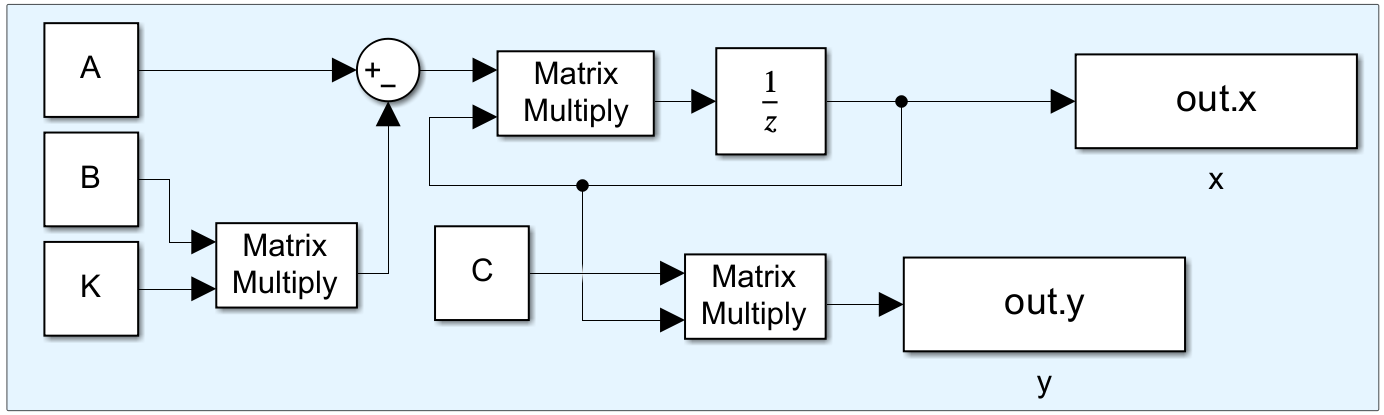
\includegraphics[width=1\linewidth]{pic/1_1_schem.png}}
	\caption{Схема моделирования.}
	\label{1_1_schem}
\end{figure}

Осуществим моделирование замкнутой системы (рисунок \ref{1_1_schem}), графики переменных вектора состояния и выходной переменной ОУ представлены на рисунках \ref{1_x} и \ref{1_y}, соответственно. Заметим, что условие оптимальности по времени выполнено, так как время переходного процесса не больше $2\cdot T$ (коэффициент 2 здесь соответствует порядку системы).
\begin{figure}[h]
	\center{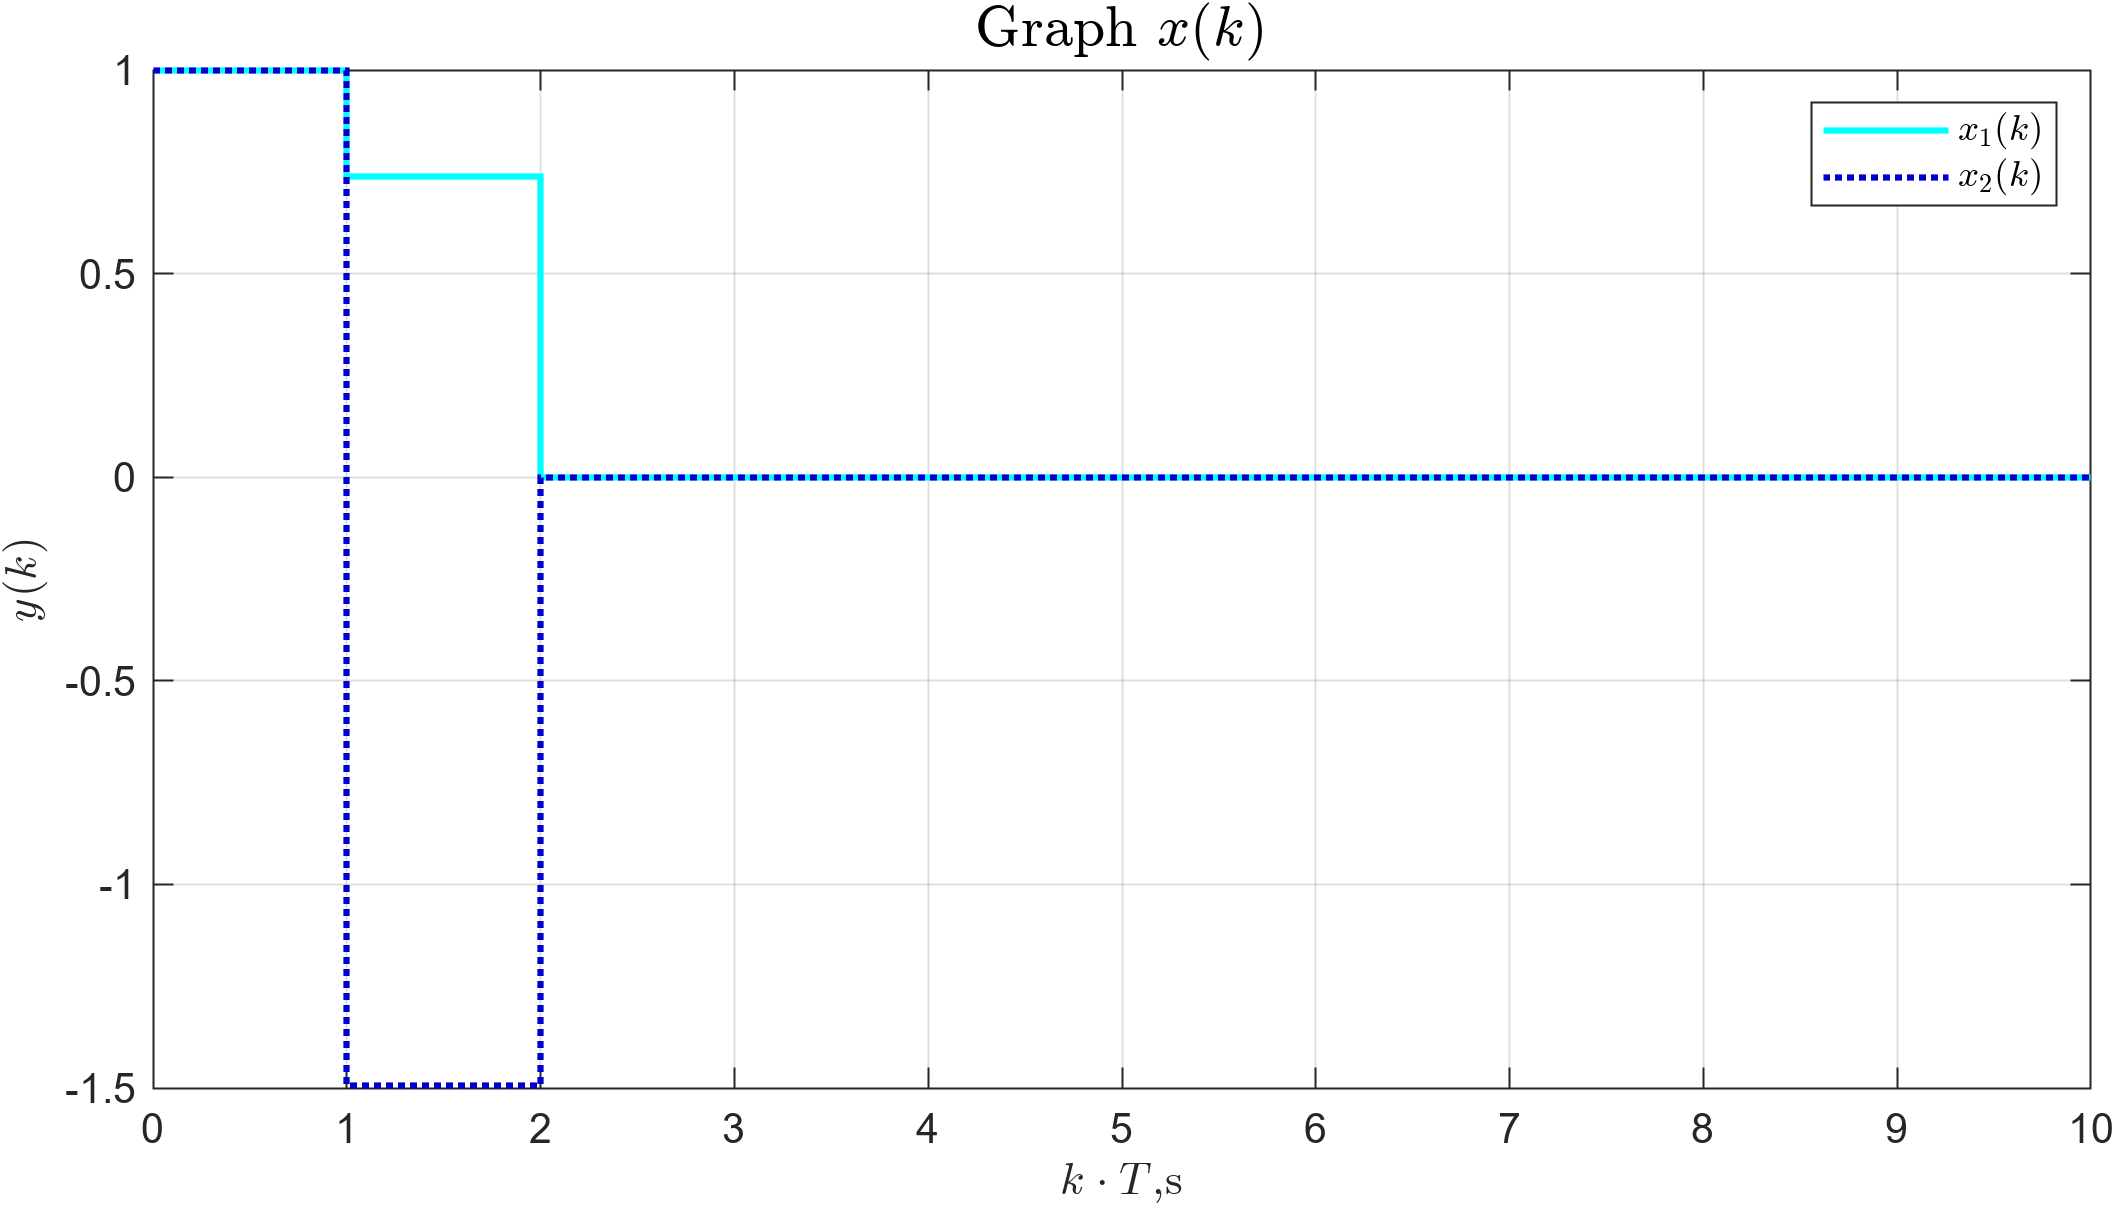
\includegraphics[width=1\linewidth]{pic/1_x.png}}
	\caption{График переменных вектора состояния $x(k)$.}
	\label{1_x}
\end{figure}
\begin{figure}[h]
	\center{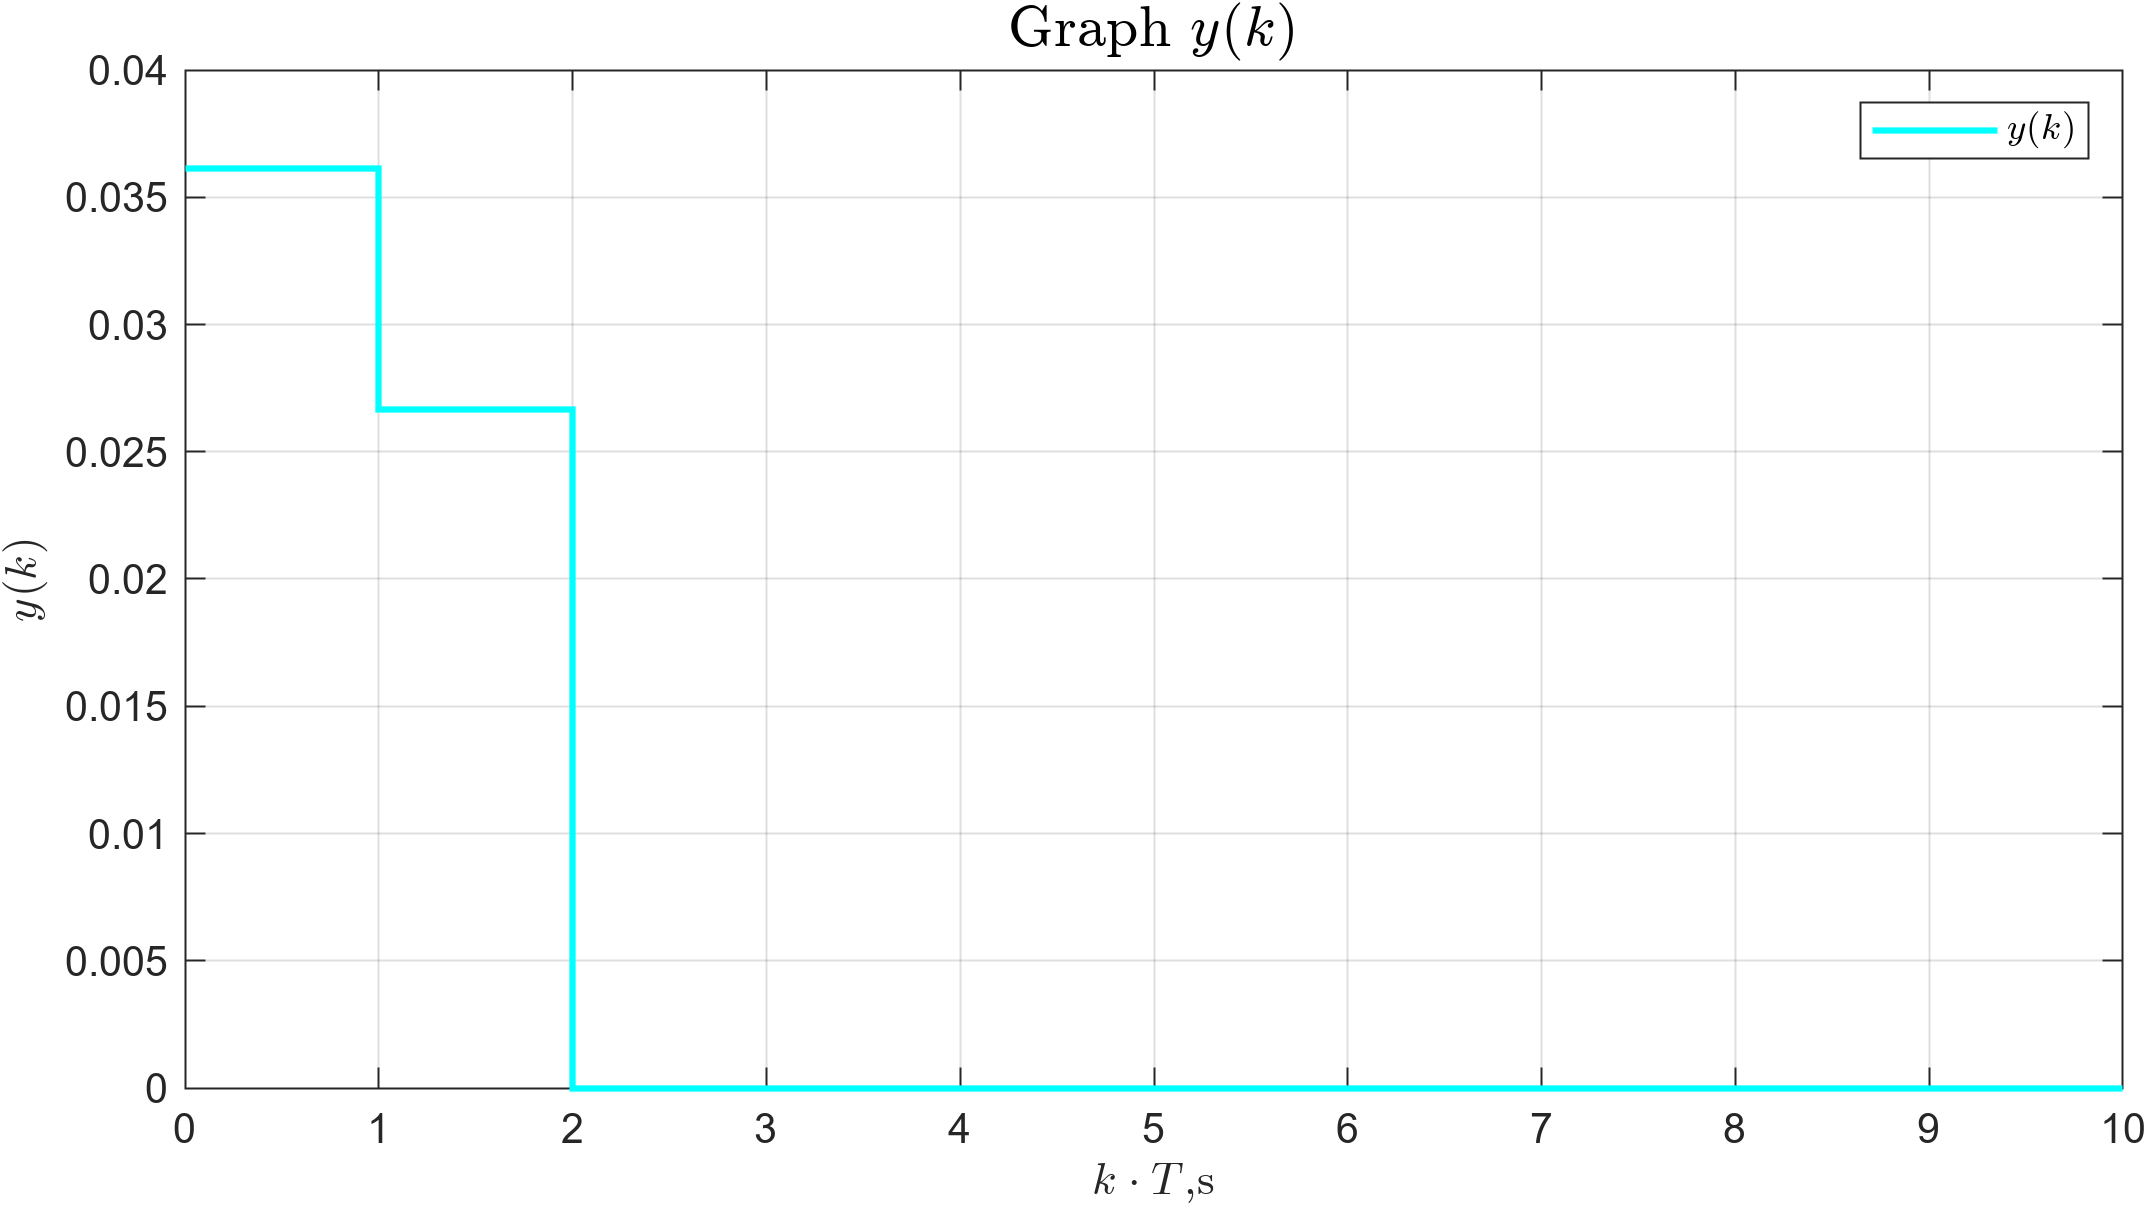
\includegraphics[width=1\linewidth]{pic/1_y.png}}
	\caption{График выходной переменной $y(k)$.}
	\label{1_y}
\end{figure}




\endinput